\documentclass[./main.tex]{subfiles}

\begin{document}

\section{Machine Learning Theory}\label{sec:theory}
Throughout this section the theory of machine learning that will be used in this thesis is described and explained. In Section \ref{subsec:motivation_theory} we describe the general motivation behind using machine learning. Then, in Section \ref{subsec:ml_paradigmes} we will be giving a brief introduction to the two most common machine learning paradigms, as well as how we will be using them. In Section \ref{subsec:evaluation}, we give a brief overview of how to evaluate a developed model. Lastly, in Section \ref{subsec:NeuralNetworks}, we describe the mathematics behind feedforward- and convolutional neural networks .

\subsection{Motivation}\label{subsec:motivation_theory}
It can be difficult for humans to recognize certain patterns and trends in data. This becomes more difficult the greater the quantity of the data is, which is becomming more and more common with the rapidly growing topic of \textit{Big Data}. For this reason, computers are often used instead of humans to recognize patterns and trends in the data by analyzing the data, which is what is called \textit{Machine Learning}. In this thesis, we will use machine learning in section \ref{experiement} to develop a model for estimating the $2$D pose of a single human in an image. Later, in section \ref{sec:XAI}, we will use machine learning to improve our understanding of the model.

\subsection{Machine Learning Paradigms}\label{subsec:ml_paradigmes}
Machine learning is usally split into the at least two paradigmes:
\begin{enumerate}
    \item \textit{Supervised learning} where the data consists of features and labels. By analyizing the data the algorithm learns to predict the labels given the features \cite{ESL}. Supervised learning is further split into \textit{classification} and \textit{regression}.
    \item \textit{Unsupervised learning} where the data only consists of features. The algorithm then learns properties of the data, without any provided labels \cite{ESL}.
\end{enumerate}
In this thesis we will make use of supervised learning when developing our model for pose estimation, where we will make use of regression. Later, unsupervised learning is used when we explore our developed model.

\subsection{Evaluation of Machine Learning Models}\label{subsec:evaluation}
When developing a machine learning model it is important to know how trustworthy the developed model is. This is usually done by testing how good the model is at generalizing to unseen data, which is done by making use of several dataset splits and \textit{evaluation metrics}.

\subsubsection{Splitting the dataset}
When developing a machine learning model, the data needs to both create the model, but also to evaluate the model. For the evaluation of the model, one of the two following techniques is usually used

\begin{enumerate}
    \item \textit{Cross validation} where the data is split into $K$ non-overlapping chunks. The model is then trained for $K$ rounds on $K - 1$ chunks, where the last chunk is used for evaluating the model \cite{MAD_book}.
    \item \textit{Train-validation-test} where the data is split into $3$ random non-overlapping chunks: $(1)$ the training dataset, $(2)$ the validation dataset, and $(3)$ the testing dataset. The training dataset is then used for training the model and the validation dataset is used for evaluating the model as it is being developed - this often means, that the \textit{hyperparameters}, the paramters that are not possible to fit from the data, are being tweaked to yield the best validation loss. Lastly, the testing dataset is used as a final evaluation of the model to yield an unbiased evaluation of the ability of the model to generalize to unseen data. Once the testing dataset has been used it can no longer be used for evaluating the data, as this potentially introduces bias in future evaluations \cite{MAD_L3}.
\end{enumerate}
Throughout this thesis the train-validation-test technique will be used over cross validation for evaluating the developed models. This will be done, since cross validation is better suited for smaller datasets, as the runtime is much greater than the runtime of the train-validation-test technique.

\subsubsection{Evaluation Metrics for Supervised Machine Learning}
\begin{algorithm}[htbp]
    \caption{PCK \cite{Camilla}\cite{SHG}}
    \label{Algorithm:PCK}
    \begin{algorithmic}[1]
        \Require Ground truth heatmaps $heatmaps_{gt}$ of keypoints
        \Require Predicted heatmaps $heatmaps_{pred}$ of keypoints
        \Require Threshold radius $r$
        \Require Normalization constant $c$
        \State Let $n = 0$ be the running total of correctly predicted keypoints
        \State Let $N \text{ be the amount of annotated heatmaps}$
        \ForAll{annotated ground truth heatmap, $heatmap_{gt}$, in $heatmaps_{gt}$}
            \State Let $(x_{gt}, y_{gt})$ be the $2D$ index of the maximum activation of $heatmap_{gt}$
            \State \begin{varwidth}[t]{\linewidth}
                Let $(x_{pred}, y_{pred})$ be the $2D$ index of the maximum activation of the predicted heatmap corresponding to $heatmap_{gt}$
            \end{varwidth}
            \State Let $dist$ be the Euclidean distance between $(x_{gt}, y_{gt})$ and $(x_{pred}, y_{pred})$.
            \State Normalize $dist$: $dist = \frac{dist}{c}$
            \If{$dist < r$}
                \State $n = n + 1$
            \EndIf
        \EndFor
        \State Let $ratio = \frac{n}{N}$ be the ratio of correctly annotated heatmaps
        \State \textbf{return} $ratio$
    \end{algorithmic}
\end{algorithm}
\noindent When we have trained a model, we need to somehow evaluate how well the model performs on unseen data. This is usually done by making use of evaluation metrics. In articulated human pose estimation, one commonly used evaluation metric is the \textit{Percentage of Correct Keypoints} (\textit{PCK}), which states the percentage of predictions that are within a normalized distance of the ground truth \cite{SHG}.
\\
\\
The pseudocode of PCK is visualized in Algorithm \ref{Algorithm:PCK}. The algorithm works by iterating over each annotated ground truth heatmap and the corresponding predicted heatmap. It then finds the distance between the maximum activation of a ground truth heatmap and the corresponding predicted heatmap. The distance is then normalized by a constant $c$ and compared to a threshold radius $r$. The ratio of the normalized distances that are less than the threshold $r$ are then computed and returned, yielding the PCK accuracy between the ground truth heatmaps and the corresponding predicted heatmaps \cite{Camilla} \cite{SHG}. The aim is thus to maximize the PCK accuracy.

\subsection{General Machine Learning Terminology}\label{subsec:general_ML_terminology}
Machine learning uses a bunch of different terminologies. The most general machine learning terminologies are explained throughout the following section.

\noindent \textbf{Loss Functions} \\
The training of a machine learning model is done by minimizing a given \textit{loss function}, which measures the error of the model. There are many different loss functions, each with their own advantages and disadvantages. One of the most common loss functions for regression is the \textit{Mean Squared Error (MSE)}, defined as
$$MSE = \frac{1}{n} \sum_{i = 1} ^n \left( y_i - \hat{y}_i \right)^2$$
where $y_i$ is the true value of the $i$th observation and $\hat{y}_i$ is the estimated value of the $i$th observation. Thus, $MSE$ measures the average squared difference between the true observation and the estimated observation \cite{ISL}. $MSE$ will we be using in Section \ref{experiement}, when we develop our model.
\\
\\
\noindent \textbf{Overfitting and Regularization} \\
The main goal of a machine learning model is to generalize well on unseen data. This can often be difficult, as the model simply "remembers" the training data instead of learning the patterns in the training data. In other words, the gap between the training error and the test error is too large, which is a concept called \textit{overfitting}. Certain techniques are designed to reduce the test error - these techniques are collectively called \textit{regurlization} \cite{DeepLearning}. One commonly used Regularization technique is \textit{batch normalization}, which we will be using when we in Section \ref{experiment} wil be developing our model. Batch normalization will be described further in Section \ref{subsec:NeuralNetworks}.
\\
\\
\textbf{Gradient Descent}
\begin{algorithm}[htbp]
    \caption{Gradient Descent \cite{d2l}}
    \label{Algorithm:gradient_descent_alg}
    \begin{algorithmic}[1]
        \Require Learning rate $\eta$
        \Require Initial parameter $\bm{\theta}$
        \While{stopping criterion not met}
            \State Sample an observation from the training set $\bm{x}$ with corresponding target $\bm{y}$
            \State Apply update: $\bm{\theta} = \bm{\theta} - \eta \nabla_{\bm{\theta}} L\left( f(\bm{x}; \bm{\theta}), \bm{y} \right)$
        \EndWhile
    \end{algorithmic}
\end{algorithm}
\newline
There are different methods for minimizing the loss function of a model during training, however, the most common algorithms are variants of \textit{gradient descent}, whose algorithm is described in Algorithm \ref{Algorithm:gradient_descent_alg}. The algorithm works by taking a learning rate $\eta$ and the initial parameter $\bm{\theta}$ as input. It then computes $\nabla_{\bm{\theta}} L\left( f(\bm{x}; \bm{\theta}), \bm{y} \right)$, which is multiplied by $\eta$ and  subtracted from $\bm{\theta}$. This is done until a stopping condition is met, such as when the magnitude of the gradient $\left|  \nabla_{\bm{\theta}} L\left( f(\bm{x}; \bm{\theta}), \bm{y} \right) \right|$ is small or until a maximum amount of iterations has been reached \cite{d2l}.
\\
\\
\noindent \textbf{Online, Mini-batch and Batch methods} \\
\noindent When gradient descent is used in machine learning, computing $\nabla_{\bm{\theta}} L\left( f(\bm{x}; \bm{\theta}), \bm{y} \right)$ can be done by averaging the gradient of each of the $n$ observations of the training set, which is called a \textit{batch gradient method} and is computational inefficient, as the cost is $\mathcal{O}(n)$. It is therefore common to use variants of gradient descents, that reduces the cost of computing the gradient. In \textit{online gradient methods} a single observation from the dataset is used to compute the gradient, which brings the cost down to $\mathcal{O}(1)$. In \textit{mini-batch gradient methods} a subset of the dataset is used to compute the gradient, making the cost $\mathcal{O}(|\mathcal{B}|)$, where $|\mathcal{B}|$ is the mini-batch size. Thus, batch gradient descent uses the fewest iterations, however, each iteration takes the longest to compute, whereas in online gradient descent each iteration is computed quickly, however, it also uses more iterations  \cite{d2l}.
\\
\\
\noindent \textbf{Optimization Algorithms}\\
\begin{algorithm}[htbp]
    \caption{Stochastic Gradient Descent with Momentum \cite{DeepLearning}}
    \label{Algorithm:SGD_momentum}
    \begin{algorithmic}[1]
        \Require Learning rate $\eta$
        \Require Momentum parameter $\alpha$
        \Require Initial parameter $\bm{\theta}$
        \Require Initial velocity $\bm{v}$
        \While{Stopping criterion not met}
            \State \begin{varwidth}[t]{\linewidth}
            Sample a minibatch of $m$ random observations from the training set $\{\bm{x}^{(1)}, ..., \bm{x}^{(n)}\}$ with corresponding targets $\bm{y}^{(i)}$
            \end{varwidth} 
            \State Compute gradient estimate: $\bm{g} = \frac{1}{m} \nabla_{\bm{\theta}} \sum_i L\left( f \left( \bm{x}^{(i)}; \bm{\theta} \right), \bm{y}^{(i)} \right)$
            \State Compute velocity update: $\bm{v} = \alpha \bm{v} - \eta \bm{g}$
            \State Apply update: $\bm{\theta} = \bm{\theta} + \bm{v}$
        \EndWhile
    \end{algorithmic}
\end{algorithm}
\begin{algorithm}[htbp]
    \caption{RMSProp \cite{DeepLearning}}
    \label{Algorithm:RMSProp}
    \begin{algorithmic}[1]
        \Require Learning rate $\eta$
        \Require Decay rate $\rho$
        \Require Starting position $\bm{\theta}$
        \Require Small constant $\delta$, usually $10^{-6}$
        \State Initialize accumulation variables $\bm{r} = \bm{0}$
        \While{stopping criterion not met}
            \State \begin{varwidth}[t]{\linewidth}
            Sample a minibatch of $m$ random observations from the training set $\{\bm{x}^{(1)}, ..., \bm{x}^{(m)}\}$ with corresponding targets $\bm{y}^{(i)}$
            \end{varwidth}
            \State Compute gradient: $\bm{g} = \frac{1}{m} \nabla_{\bm{\theta}} \sum_i L\left( f \left(\bm{x}^{(i)}; \bm{\theta} \right), \bm{y}^{(i)} \right)$
            \State Accumulate squared gradient: $\bm{r} = \rho \bm{r} + (1 - \rho) \bm{g} \odot \bm{g}$
            \State Compute parameter update: $\Delta\bm{\theta} = - \frac{\eta}{\sqrt{\delta + \bm{r}}} \odot \bm{g}$. \quad ($- \frac{1}{\sqrt{\delta + \bm{r}}}$ applied element-wise)
            \State Apply update: $\bm{\theta} = \bm{\theta} + \Delta \bm{\theta}$ 
        \EndWhile
    \end{algorithmic}
\end{algorithm}
\newline
An example of a mini-batch based optimization algorithm is \textit{Stochastic Gradient Descent} (\textit{SGD}). SGD is very closely related to the algorithm behind gradient descent, however, instead of updating the parameters for each sample, SGD instead uses the mean gradient of $n$ randomly selected samples to update its parameters.
\\
\\
\noindent One problem of the gradient descent algorithm is, that the learning rate can be difficult to choose. Therefore, there have been developed a range of various optimization algorithms that uses a separate learning rate for each parameter and automatically adapt these learning rates. One of which is \textit{RMSProp}, which is visualized in Algorithm \ref{Algorithm:RMSProp}. The algorithm works by using an decaying average that discards knowledge from the extreme past, so that it can converge after finding a convex bowl of the loss function. The algorithm uses a hyperparameter $\rho$, that controls the length scale of the moving average \cite{DeepLearning}.
\\
\\
\textbf{Momentum} \\
One problem with SGD is how slow it often can be. For this reason \textit{momentum} is often used to accelerate learning. Momentum works by accumulating a decaying moving average of the past gradients and continuing to move in their direction. This is done by introducing two new variable; $\bm{v}$, which is the direction and speed of which the parameters move through the parameter space, and $\alpha \in [0, 1)$, which describes how quickly the contribution of previous gradients decay. Common values of $\alpha$ are $0.5, 0.9$ and $0.99$ \cite{DeepLearning}. 
\\
\\
\textbf{Epoch} \\
An \textit{epoch} is an iteration through the complete dataset during fitting of the network. Multiple epochs are often needed to reach the minimum of the loss function \cite{d2l}.

\subsection{Neural Networks} \label{subsec:NeuralNetworks}
In recent years \textit{deep learning} and \textit{neural networks} have revolutionized the use of machine learning. In this thesis a neural network will be used for performing the human pose estimation. Throughout subsection \ref{subsec:NeuralNetworks} the theory and mathematics behind neural networks is described and explained.
\subsubsection{Feedforward Neural Networks} \label{subsubsec:FeedforwardNN}
\begin{figure}[htbp]
    \centering
    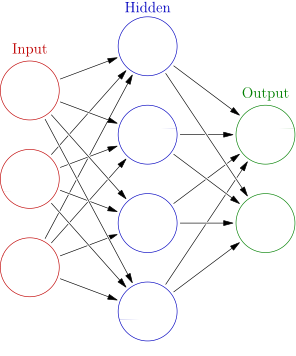
\includegraphics[height = 5 cm]{entities/feed_forward_nn.jpg}
    \caption{Visualization of a feedforward neural network with a single hidden layer \cite{feedforward_nn}}
    \label{feedforward_nn}
\end{figure}
\noindent \textbf{The Architecture and Forwardpropagation} \\
One of the most common types of neural networks are \textit{feedforward neural networks}, where the data flows unidirectionally through the network. Such a network is visualized in Figure \ref{feedforward_nn}. The network is a directed acyclic graph and is built up of three types of components: the \textit{input layer}, the \textit{hidden layers} and the \textit{output layer}. Each layer is built up of \textit{units}, also called \textit{neurons} (which are visualized as circles in Figure \ref{feedforward_nn}), where each neuron has a \textit{bias} assigned to it, and is connected to one or two other layers through \textit{edges} (which are visualized as arrows in Figure \ref{feedforward_nn}), where each edge has a \textit{weight} assigned to it. Hidden layers are connected to two other layers - one before the hidden layer and one after the hidden layer - where the input layer is only connected to the next layer in the network and the output layer is only connected to the previous layer in the network. 
\\
\\
We can define the network mathemaically by letting $a_n ^{(i)}$ denote the value of the $n$th node in the $i$th layer, $w_{m, n}$ denote the value of the weight of the edge connecting the $n$th node in the $i$th layer to the $m$th node in layer $i + 1$ and $b_n ^{(i)}$ denote the bias corresponding to the $n$th node in the $i$th layer. \\
When data flows through the model it follows the following formula
$$\bm{a}^{(i + 1)} = g^{(i + 1)} \left( \bm{z}^{(i + 1)} \right)$$
where
$$\bm{z}^{(i + 1)} = \bm{W}^{(i + 1)} \bm{a}^{(i)} + \bm{b}^{(i + 1)},$$
$\bm{W}^{(i + 1)}$ is the weights between layer $i$ and layer $i + 1$ defined by
\begin{center}
    \begin{math}
        \bm{W}^{(i + 1)} =
        \begin{pmatrix}
            w_{0, 0} & w_{0, 1} & \cdots & w_{0, n} \\
            w_{1, 0} & w_{1, 1} & \cdots & w_{1, n} \\
            \vdots & \vdots & \ddots & \vdots \\
            w_{m, 0} & w_{m, 1} & \cdots & w_{m, n}
        \end{pmatrix}
        ,
    \end{math}
\end{center}
$\bm{a}^{(i)}$ is the values of the nodes in the $i$th layer defined by
\begin{center}
    \begin{math}
        \bm{a}^{(i)} =
        \begin{pmatrix}
            a_{0} ^{(i)} \\
            a_{1} ^{(i)} \\
            \vdots \\
            a_{n} ^{(i)} \\
        \end{pmatrix}
        ,
    \end{math}
\end{center}
$\bm{b}^{(i + 1)}$ is the values of the biases of layer $i + 1$ defined by
\begin{center}
    \begin{math}
        \bm{b}^{(i + 1)} =
        \begin{pmatrix}
            b_{0} ^{(i + 1)} \\
            b_{1} ^{(i + 1)} \\
            \vdots \\
            b_{m} ^{(i + 1)} \\
        \end{pmatrix}
    \end{math}
\end{center}
and $g$ is a non-linear \textit{activation function}, that is typically applied element-wise \cite{DeepLearning} \cite{3b1b_1}. The purpose behind using non-linear activation functions is to make it possible for the output of the network to be non-linear. One often used activation function is the \textit{rectified linear activation function} (or \textit{ReLU} for short) defined by
$$g(x) = \max\{0, x\}.$$
The ReLU-function is very close to being linear, making the function keep many of the properties of linear functions that make them easy to optimize and generalizing, which are two great advantages of using the ReLU-function. Another great advantage of using the ReLU-function is stated by the \textit{universal approximation theorem} which states, that a feedforward network with a linear output layer and at least one hidden layer with the ReLU-function (or another non-linear activation function from a wide class of activation functions) can approximate any continuous function on a closed and bounded subset of $\mathbb{R}^n$ (and actually some functions outside of this class), as long as the network has enough hidden neurons \cite{DeepLearning}. 
\\
\\
\noindent \textbf{Backpropagation} \\
Backpropagation is an algorithm used to compute the gradient of the network. It is used together with an optimization algorithm to train the model by minimizing the training loss of the model. Backpropagation happens after data has flowed through the model from the input to the output, and works by computing the gradient of each parameter sequentially from the output to the input of the model, using the chain rule \cite{DeepLearning}. By using the chain-rule we find, that the partial derivative of the loss $L$ for each weight is
$$\frac{\partial L}{\partial w_{jk} ^{(i)}} = \frac{\partial z_j ^{(i)}}{\partial w_{jk} ^{(i)}} \frac{\partial a_j ^{(i)}}{\partial z_j ^{(i)}} \frac{\partial L}{\partial a_j ^{(i)}} = a_k ^{(i - 1)} g ^{\prime (i)} \left( z_j ^{(i)} \right) \frac{\partial L}{\partial a_j ^{(i)}}$$
and the partial derivative of each bias is
$$\frac{\partial L}{\partial b^{(i)} _j} = \frac{\partial z^{(i)} _j}{\partial b^{(i)} _j} \frac{\partial a_j ^{(i)}}{\partial z^{(i)} _j} \frac{\partial L}{\partial a_j ^{(i)}} = g^{\prime (i)} \left( z_j ^{(i)} \right) \frac{\partial L}{\partial a_j ^{(i)}}$$
where for both cases
$$ \frac{\partial L}{\partial a_j ^{(i)}} = \sum_{j = 0} ^{n_i - 1} w_{jk} ^{(i + 1)} g^{\prime (i + 1)} \left( z_j ^{(i + 1)} \right) \frac{\partial L}{\partial a_j ^{(i + 1)}}.$$
if $\bm{a}^{(i)}$ is not the output-layer. Once the partial derivative of all weights and biases has been found, the gradient vector can be formed and an optimization method can be used to optimize the parameters of the model \cite{3b1b_4}.
\\
\\
\textbf{Batch Normalization} \\
\textit{Batch normalization} is a reparametrization method, which is applied to individual layers in a neural network. If $\bm{x} \in \mathcal{B}$ is an input to the batch normalization, $\text{BN}$, then batch normalization is done by the following
$$\text{BN}(\bm{x}) = \bm{\gamma} \odot \frac{\bm{x} - \hat{\bm{\mu}}_{\mathcal{B}}}{\hat{\bm{\sigma}}_{\mathcal{B}}} + \bm{\beta}$$
where
$$\hat{\bm{\mu}}_{\mathcal{B}} = \frac{1}{|\mathcal{B}|} \sum_{\bm{x} \in \mathcal{B}} \bm{x}$$
and
$$\hat{\bm{\sigma}}_{\mathcal{B}} = \sqrt{\frac{1}{|\mathcal{B}|} \sum_{\bm{x} \in \mathcal{B}} \left(\bm{x} - \hat{\bm{\mu}}_{\mathcal{B}} \right)^2 + \epsilon},$$
which makes the minibatch have $0$ mean and unit variance, where the small constant $\epsilon > 0$ is simply used to avoid division by zero. $\bm{\gamma}$ and $\bm{\beta}$ are often trainable parameters, that are used to make the mini-batch have an arbitrary mean and standard deviation and have the same shape as $\bm{x}$. This helps the network to converge, as the batch normalization keeps centering the mean and standard deviation of the mini-batches \cite{d2l}.

\subsubsection{Convolutional Neural Networks} \label{subsubsec:CNN}
\begin{figure}[htbp]
    \centering
    \begin{subfigure}[t]{0.4\textwidth}
        \centering
        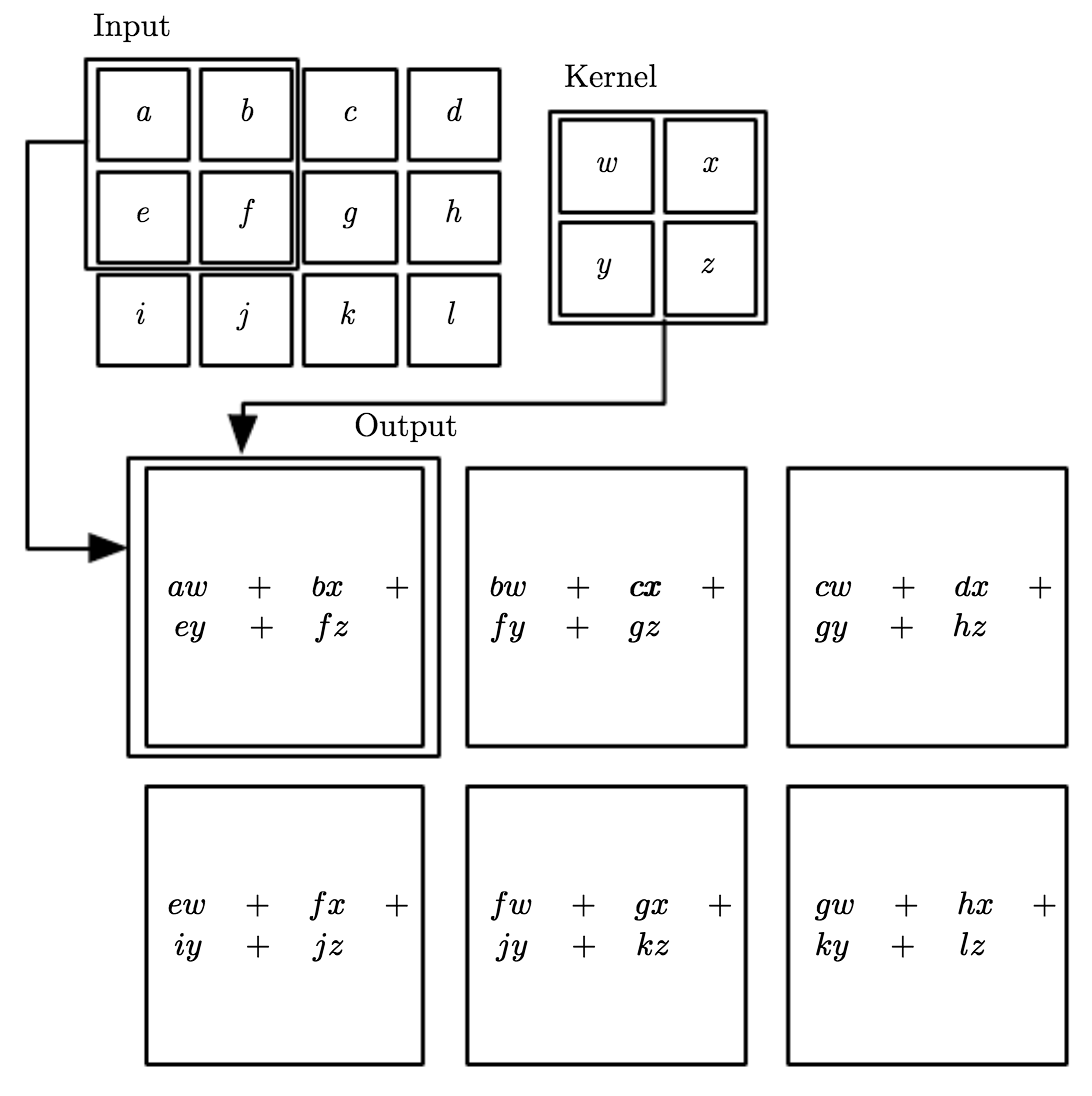
\includegraphics[height = 6 cm]{entities/2d_convolution_example.png}
        \caption{Example of a 2D convolution \cite{DeepLearning}}
    \end{subfigure}
    \begin{subfigure}[t]{0.4\textwidth}
        \centering
        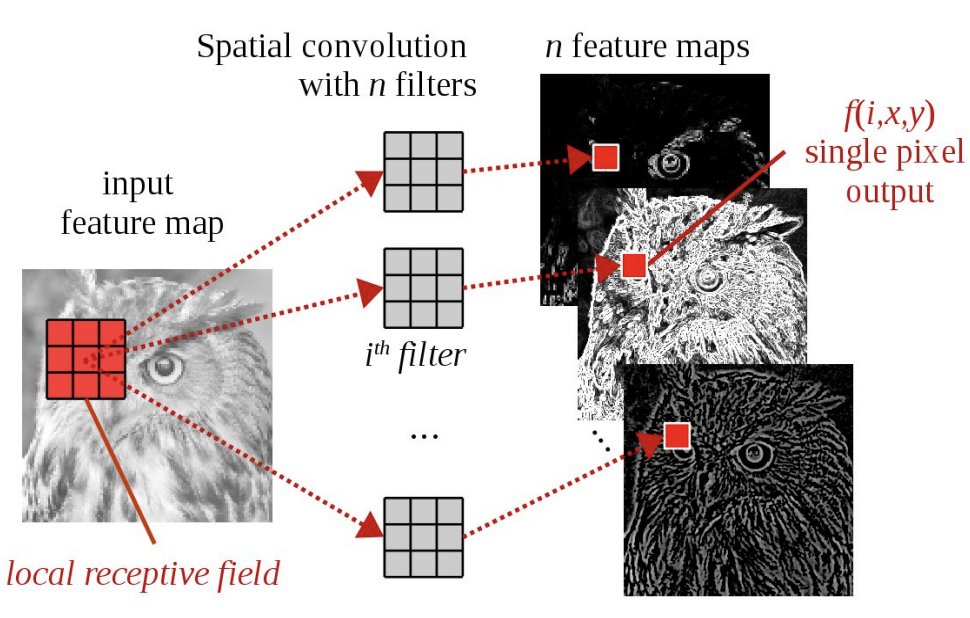
\includegraphics[height = 5 cm]{entities/3d_convolution_example.png}
        \caption{Example of a convolution with multiple filters \cite{Everything}}
    \end{subfigure}
    \caption{Convolutions visualized}
    \label{fig:convolutionexample}
\end{figure}
\noindent Feedforward neural networks introduced in \ref{subsubsec:FeedforwardNN} can be used for pattern recognition within images, however, they are usually not used for this task. Consider a colored input image with $3$ channels of dimension $64 \times 64$. If we were to use a feedforward neural network on this image, each neuron in the first hidden layer would be connected to the input layer through $12.288$ weights. Not only would this use a lot of computational power and time to train, however, a network of this size would also be prone to overfitting. Instead, \textit{convolutional neural networks} (also known as \text{CNN}'s) are usually used \cite{CNN}, which dramatically reduces the amount of weights used. In addition, by using a CNN the high correlation between a pixel and its neighbours are also captured, essentially leading to better results. A CNN usually consists of \textit{convolutional layers}, \textit{pooling layers} and \textit{fully-connected layers}, where the fully-connected layers are analogous to the layers in a feedforward neural network.
\\
\\
\textbf{Convolutional layers} \\
A convolutional layer is composed of a set of \textit{kernels} (also known as \textit{filters}), which are matrices of weights of dimension $c \times k \times k$, where $c$ is the amount of channels (or amount of filters to be applied) and $k$ kernel-size, usually $5$, $3$ or $1$. The convolutional layer thus consists of $c$ filters, each of $k \times k$ parameters, where each weight is a parameter for the model to be learned \cite{Everything}. Each kernel is used on the input to produce a \textit{feature map}. The kernels are applied to the input by "sliding" over the input (where the step size is called \textit{stride}). Each $k \times k$ grid of the input (called the \textit{local receptive field}) is then used to compute the dot-product between the grid and each kernel, which is then placed in the corresponding feature map of each kernel, as visualized in Figure \ref{fig:convolutionexample}. When all of the feature maps have been computed, an activation function can be applied.
\\
\\
\textbf{Pooling layers}\\
Pooling layers are layers used to reduce the dimension of the input. The most common pooling layer is the \textit{maxpooling}-operation. The operation works by considering each $k \times k$ local receptive field, in which the maximum entry is being inserted into the output \cite{CNN}.
\\
\\
\noindent \textbf{Nearest Neighbour Upsampling}
\begin{algorithm}[htbp]
    \caption{Nearest Neighbour Upsampling \cite{NNUpsampling}}
    \label{Algorithm:NNUpsampling}
    \begin{algorithmic}[1]
        \Require Input image $X$ of size $m \times n$
        \Require Wanted output size $xm \times yn$, where $x, y \in \mathbb{Z}^{+}$
        \State Create empty image $O$ of size $xm \times yn$
        \ForAll{pixel $p \in X$}
            \State $i,j = \text{index of } p \text{ in } X$
            \State Insert $p$ at index $(xi, yj)$ in $O$
        \EndFor
        \ForAll{empty pixel $p \in O$}
            \State Let $p$ be the value of the nearest neighbour
        \EndFor
        \State \textbf{return} $O$
    \end{algorithmic}
\end{algorithm}
\newline
Sometimes we want to increase the size of an image. This can be done by making use of \textit{upsampling} (also known as \textit{interpolation}) techniques. One of the most common upsampling techniques is \textit{nearest neighbour upsampling}, whose pseudocode has been written in Algorithm \ref{Algorithm:NNUpsampling}. The algorithm starts off by taking an image, $X$, of size $m \times n$, as input, which we wish to upsample to size $xm \times yn$, where $x$ and $y$ are positive whole numbers. The algorithm then loops over each pixel $p \in X$, finds the corresponding index $(i, j)$, of $p$ in $X$, and places $p$ at index $(xi, yj)$ in the output image $O$ of size $xm \times yn$. When this is done, it assigns each of the empty pixel in $O$ the value of their nearest neighbour and returns $O$ \cite{NNUpsampling}.

\end{document}